\documentclass{article}

\usepackage{amsmath}
\usepackage{amssymb}
\usepackage{parskip}
\usepackage{fullpage}
\usepackage{hyperref}
\usepackage{tikz}

\usepackage[backend=bibtex]{biblatex}

\addbibresource{resources/references.bib}

\usetikzlibrary{angles,quotes}

\hypersetup{
    colorlinks=true,
    linkcolor=black,
    urlcolor=blue,
    pdftitle={Physical Rendering},
    pdfpagemode=FullScreen,
}

\title{Physical Rendering}
\author{Paolo Bettelini}
\date{}

\begin{document}

\maketitle
\tableofcontents
\pagebreak

\section{Measurements}

\subsection{Radiant Flux}

The radiant flux (or power) \(\Phi\) is the total amount of energy passing
through a surface per second and is measured in \([W]\) (watts) as \(\frac{J}{s}\).

\subsection{Irradiance}

The irradiance \(E\) is the measurements of the radiant flux per \textit{unit area}
and is measured in \([W]{[M]}^{-2}\) as \(\frac{\Phi}{m^2}\).

\subsection{Radiance}

The radiance \(L\) is the irradiance per unit solid angle (steradian) and is
measured in \([W]{[M]}^{-2}{[sr]}^{-1}\) as \(\frac{E}{sr}\).

\section{Geometry}

\subsection{Fundamental vectors}

% tikz picture
\begin{center}
    \begin{tikzpicture}
        \draw (-4,0) -- (4, 0);
        \draw (0,0) coordinate (a) -- (-3, 3) coordinate (b);
        \draw[->] (a) -- (0, 3) coordinate (c);
        \draw[->] (a) -- (3, 3) coordinate (d);

        \node[below] at (a) {\(x\)};
        \node[right] at (d) {\({\hat{V}}^t\)};
        \node[left] at (b) {\(\hat{V}\)};
        \node[left] at (c) {\(\hat{N}\)};
        \node[right] at (c) {\(\hat{L},\hat{R}\)};

        \pic["\({\theta}_r\)", draw=black, -, angle eccentricity=1.2, angle radius=1cm] {angle=d--a--c};
        \pic["\({\theta}_i\)", draw=black, -, angle eccentricity=1.2, angle radius=1cm] {angle=c--a--b};
    \end{tikzpicture}
\end{center}

\begin{itemize}
    \item \(\hat{V}\) direction torwards the camera
    \item \(\hat{N}\) surface normal
    \item \(\hat{L}\) vector pointing torward the light source
    \item \(\hat{R}\) reflected ray direction
    \item \({\theta}_i, {\theta}_r\) incident and reflected angles
\end{itemize}

The reflected ray is given by \(\hat{R}=\hat{L}-2\hat{N}(\hat{L}\cdot\hat{N})\)

\subsection{Light attenuation}

The amount of radiance on a point is given by
\[
    \Phi \left(\hat{L} \cdot \hat{N}\right) = \Phi \cdot \cos(\alpha)
\]
where \(\alpha\) is the angle between the two vectors.
\\
This means that if the light source is perfectly above the point, then
there is not light attenuation \((\alpha = 0)\).

\pagebreak

\section{Materials}

\subsection{Types of materials}

Different materials reflect incoming light to different directions and absord different amounts of it.

\begin{center}
    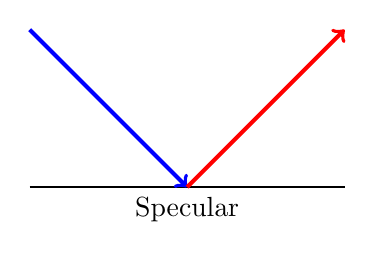
\begin{tikzpicture}[scale=2]
        % surface
        \draw[line width=0.25mm] (-1,0) -- (1, 0);

        % ray in
        \draw[->][line width=0.5mm, color=blue] (-1,1) -- (0, 0);

        % rays out
        \draw[->][line width=0.5mm, color=red] (0,0) -- (1, 1);

        % label
        \node[below] at (0,0) {Specular};
    \end{tikzpicture}
    \qquad
    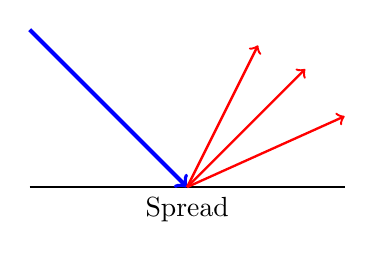
\begin{tikzpicture}[scale=2]
        % surface
        \draw[line width=0.25mm] (-1,0) -- (1, 0);

        % ray in
        \draw[->][line width=0.5mm, color=blue] (-1,1) -- (0, 0);
        
        % rays out
        \draw[->][line width=0.3mm, color=red] (0,0) -- (0.75, 0.75);
        \draw[->][line width=0.3mm, color=red] (0,0) -- (0.45, 0.9);
        \draw[->][line width=0.3mm, color=red] (0,0) -- (1, 0.45);

        % label
        \node[below] at (0,0) {Spread};
    \end{tikzpicture}
    \qquad
    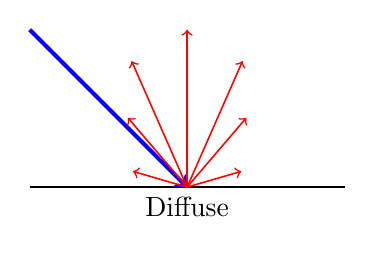
\begin{tikzpicture}[scale=2]
        % surface
        \draw[line width=0.25mm] (-1,0) -- (1, 0);

        % ray in
        \draw[->][line width=0.5mm, color=blue] (-1,1) -- (0, 0);
        
        % rays out
        \draw[->][line width=0.2mm, color=red] (0,0) -- (0.376, 0.44);
        \draw[->][line width=0.2mm, color=red] (0,0) -- (-0.376, 0.44);
        \draw[->][line width=0.2mm, color=red] (0,0) -- (0.352, 0.8);
        \draw[->][line width=0.2mm, color=red] (0,0) -- (-0.352, 0.8);
        \draw[->][line width=0.2mm, color=red] (0,0) -- (0.344, 0.1);
        \draw[->][line width=0.2mm, color=red] (0,0) -- (-0.344, 0.1);
        \draw[->][line width=0.2mm, color=red] (0,0) -- (0, 1);

        % label
        \node[below] at (0,0) {Diffuse};
    \end{tikzpicture}
\end{center}

\subsection{Bidirectional reflectance distribution function}

The BRDF function (Bidirectional reflectance distribution function) is a probability distribution
for the amount of light reflected in a certain direction.
\[
    f_r(\hat{w}, x, \hat{w}^t)
\]

\begin{itemize}
    \item \(\hat{w}\) incoming ray direction
    \item \(x\) point of collision
    \item \(\hat{w}^t\) outgoing ray direction
\end{itemize}

This function follows the Helmholtz-reciprocity
\[
    \forall \hat{w},x,\hat{w}^t, \quad f_r(\hat{w}, x, \hat{w}^t) = f_r(\hat{w}^t, x, \hat{w})
\]
positivity
\[
    \forall \hat{w},x,\hat{w}^t, \quad f_r(\hat{w}, x, \hat{w}^t) \geq 0
\]
and energy conservation
\[
    \int_\Omega f_r(\hat{w}, x, \hat{w}^t) \cos \theta \, d\hat{w}^t \leq 1
\]
where \(\Omega\) encloses the scene (usually a hemisphere).

\subsection{Bidirectional transmittance distribution function}

If the material can also transfer light through itself, we use the BTDF function
(Bidirectional transmittance distribution function).

\subsection{Bidirectional scattering distribution function}

We use the BSDF (Bidirectional scattering distribution function)
to generalize both the BTDF and BRDF.

\pagebreak

\section{Rendering equation}

The rendering equation tells us how much radiance is exiting a \textit{surface point}
in a given direction
\[
    \textit{Light exiting point} = \textit{Material emitted light} + \textit{Reflected incoming light}
\]
Formally,
\[
    L_o(x, \vec{\omega})
    =L_e(x, \vec{\omega})
    +\int_\Omega L_i(x,\vec{\omega})f_r(\vec{\omega}, x, \vec{\omega}^t)
    \cos \theta d\vec{\omega}^t
\]

\begin{itemize}
    \item \(L_o\) exiting radiance
    \item \(L_o\) emitted radiance
    \item \(\Omega\) scene
    \item \(L_i\) incoming radiance
    \item \(f_r\) BRDF
    \item \(\cos \theta\) light attenuation
\end{itemize}

This value is difficult to compute. For each point, the light at that point
depends on the incoming radiance of every other point, which also depends on the first point.
This integral is infinite-dimensional because of the infinite bounces.

% https://youtu.be/4gXPVoippTs?list=PLujxSBD-JXgnGmsn7gEyN28P1DnRZG7qi&t=1020

\pagebreak

ASSETS TO USE


The Fresnel Equation

\[
    R_s(\theta) =
        \left|
            \frac
            {
                n_1\cos \theta - n_2 \sqrt{1-{\left(\frac{n_1}{n_2}\sin \theta\right)}^2}
            }
            {
                n_1\cos \theta + n_2 \sqrt{1-{\left(\frac{n_1}{n_2}\sin \theta\right)}^2}
            }
        \right|
\]

Snell's law

\[
    \frac{\sin \theta_1}{\sin \theta_2}
    = \frac{V_1}{V_2}
    = \frac{n_2}{n_1}
\]

\pagebreak

\nocite{*} % cite all entries

\printbibliography

\end{document}
